\documentclass[preprint,authoryear]{elsarticle}
%\usepackage{natbib}
\usepackage{agda}
\usepackage{revsymb}
\usepackage{semantic}
\usepackage{graphicx}
\usepackage{url}
\renewcommand\UrlFont{\color{blue}\rmfamily}
\usepackage{stix}
\usepackage{amsmath,amssymb,amsthm}
\newtheorem{theorem}{Theorem}
\usepackage{mathpazo}
\usepackage[mathpazo]{flexisym}

\begin{document}

\title{Programming Language Foundations in Agda}

\author[adr1]{Wen Kokke}
\ead{wen.kokke@ed.ac.uk}
\author[adr2]{Jeremy G. Siek}
\ead{jsiek@indiana.edu}
\author[adr1]{Philip Wadler\corref{cor1}}
\ead{wadler@inf.ed.ac.uk}
\cortext[cor1]{Corresponding author}

\address[adr1]{University of Edinburgh, 10 Crichton Street, EH8 9AB, Edinburgh}
\address[adr2]{Indiana University, 700 N Woodlawn Ave, Bloomington, IN 47408, USA}

\begin{abstract}

  One of the leading textbooks for formal methods is \emph{Software
    Foundations} (SF), written by Benjamin Pierce in collaboration
  with others, and based on Coq. After five years using SF in the
  classroom, we came to the conclusion that Coq is not the best
  vehicle for this purpose, as too much of the course needs to focus
  on learning tactics for proof derivation, to the cost of learning
  programming language theory.  Accordingly, we have written a new
  textbook, \emph{Programming Language Foundations in Agda}
  (PLFA). PLFA covers much of the same ground as SF, although it is
  not a slavish imitation.

  What did we learn from writing PLFA? First, that it is possible. One
  might expect that without proof tactics that the proofs become too
  long, but in fact proofs in PLFA are about the same length as those
  in SF. Proofs in Coq require an interactive environment to be
  understood, while proofs in Agda can be read on the page.  Second,
  that constructive proofs of preservation and progress give immediate
  rise to a prototype evaluator. This fact is obvious in retrospect
  but it is not exploited in SF (which instead provides a separate
  normalise tactic) nor can I find it in the literature.  Third, that
  using raw terms with a separate typing relation is far less
  perspicuous than using inherently-typed terms. SF uses the former
  presentation, while PLFA presents both; the former uses about 1.6 as
  many lines of Agda code as the latter, roughly the golden ratio.

  The textbook is written as a literate Agda script, and can be found
  here:
  \begin{center}
    \url{http://plfa.inf.ed.ac.uk}
  \end{center}
\end{abstract}

\begin{keyword}
  Agda \sep Coq \sep lambda calculus \sep dependent types.  
\end{keyword}

\maketitle

\section{Introduction}

The most profound connection between logic and computation is a pun.
The doctrine of Propositions as Types asserts that a certain kind of formal
structure may be read in two ways: either as a proposition in logic or
as a type in computing.  Further, a related structure may be read as
either the proof of the proposition or as a programme of the
corresponding type.  Further still, simplification of proofs
corresponds to evaluation of programs.

Accordingly, the title of this paper, and the corresponding textbook,
\emph{Programming Language Foundations in Agda} (hence, PLFA)
also has two readings.  It may be parsed as ``(Programming Language)
Foundations in Agda'' or ``Programming (Language Foundations) in
Agda''---specifications in the proof assistant Agda both describe
programming languages and are themselves programmes.

Since 2013, one of us (Philip) has taught a course on Types and Semantics for
Programming Languages to fourth-year undergraduates and masters
students at the University of Edinburgh.  An earlier version of that
course was based on \emph{Types and Programming Languages} by
\citet{Pierce-2002}, but this version was taught from its successor,
\emph{Software Foundations} (hence, SF) by \citet{Pierce-et-al-2010},
which is based on the proof assistance Coq \citep{Huet-et-al-1997}.
We are convinced by the claim of \citet{Pierce-2009}, made in his ICFP
Keynote \emph{Lambda, The Ultimate TA}, that basing a course around a
proof assistant aids learning.

However, after five years of experience, Phil came to the conclusion
that Coq is not the best vehicle.  Too much of the course needs to
focus on learning tactics for proof derivation, to the cost of
learning the fundamentals of programming language theory.  Every
concept has to be learned twice: e.g., both the product data type, and
the corresponding tactics for introduction and elimination of
conjunctions.  The rules Coq applies to generate induction hypotheses
can sometimes seem mysterious.  While the \texttt{notation} construct
permits pleasingly flexible syntax, it can be confusing that the same
concept must always be given two names, e.g., both
\texttt{subst~N~x~M} and \texttt{N~[x~:=~M]}.  Names of tactics are
sometimes short and sometimes long; naming conventions in the standard
library can be wildly inconsistent.  \emph{Propositions as types} as a
foundation of proof is present but hidden.

We found ourselves keen to recast the course in Agda \citep{Bove-et-al-2009}.
In Agda, there is
no longer any need to learn about tactics: there is just
dependently-typed programming, plain and simple. Introduction is
always by a constructor, elimination is always by pattern
matching. Induction is no longer a mysterious separate concept, but
corresponds to the familiar notion of recursion. Mixfix syntax is
flexible while using just one name for each concept, e.g.,
substitution is \texttt{\_[\_:=\_]}. The standard library is not perfect, but
there is a fair attempt at consistency. \emph{Propositions as types} as a
foundation of proof is on proud display.

Alas, there is no textbook for programming language theory in
Agda.  \emph{Verified Functional Programming in Agda} by \citep{Stump-2016}
covers related ground, but focuses more on programming with dependent
types than on the theory of programming languages.

The original goal was to simply adapt \emph{Software Foundations},
maintaining the same text but transposing the code from Coq to Agda.
But it quickly became clear that after five years in the
classroom Philip had his own ideas about how to present the material.  They
say you should never write a book unless you cannot \emph{not} write the
book, and Philip soon found that this was a book he could not not
write.

Philip considered himself fortunate that his student, Wen, was
keen to help.  She guided Philip as a newbie to Agda and provided an
infrastructure for the book that we found easy to use and produces
pages that are a pleasure to view.  The bulk of the first draft of the
book was written January--June 2018, while Philip was on sabbatical in
Rio de Janeiro.  After the first draft was published, Jeremy wrote
eight additional chapters, covering aspects of operational and
denotational semantics.

This paper is a personal reflection, summarising what was learned in the
course of writing the textbook. Some of it reiterates advice that is
well-known to some members of the dependently-typed programming
community, but which deserves to be better known.  The paper is
organised as follows.

Section~2 outlines the
topics covered in PLFA, and notes what is omitted.  

Section~3 compares Agda and Coq as vehicles for pedagogy.  Before
writing the book, it was not obvious that it was even possible;
conceivably, without tactics some of the proofs might
balloon in size. In fact, it turns out that for the results in PLFA
and SF, the proofs are of roughly comparable size, and (in our opinion)
the proofs in PLFA are more readable and have a pleasing visual
structure.

Section~4 observes that constructive proofs of progress and
preservation combine trivially to produce a constructive evaluator for
terms.  This idea is obvious once you have seen it, yet we cannot
find it described in the literature.

Section~5 claims that raw terms should be avoided in favour of
inherently-typed terms.  PLFA develops lambda calculus with both raw
and inherently-typed terms, permitting a comparison.  It turns out the
former is less powerful---it supports substitution only for closed
terms---but significantly longer---about 1.6 times as many lines of code,
roughly the golden ratio.

Section~6 describes experience teaching from the textbook.  The point
of proof is perfection, and it turns out that an online final
examination with access to a proof assistant can lead to flawless
student performance.

Section~7 outlines our experience publishing the book as open source
in GitHub.  We were surprised at how effective this was at eliciting
community participation.  A large number of people have submitted pull
requests to improve the book.

We argue that Agda has advantages over Coq for
pedagogic purposes.  Our focus is purely on the case of a proof assistant
as an aid to \emph{learning} formal semantics using examples of
\emph{modest} size.  We admit up front that
there are many tasks for which Coq is better suited than Agda.
A proof assistant that supports tactics, such as Coq or Isabelle,
is essential for formalising serious mathematics,
such as the Four-Colour Theorem \citep{Gonthier-2008},
the Odd-Order Theorem \citep{Gonthier-et-al-2013},
or Kepler's Conjecture \citep{Hales-et-al-2017},
or for establishing correctness of software at scale,
as with the CompCert compiler \citep{Leroy-2009,Kastner-et-al-2017}
or the SEL4 operating system \citep{Klein-2009,O'Connor-2016}.

\section{Scope}

PLFA is aimed at students in the last year of an undergraduate
honours programme or the first year of a master or doctorate degree.
It aims to teach the fundamentals of operational semantics of
programming languages, with simply-typed lambda calculus as the
central example.  The textbook is written as a literate script in Agda.
As with SF, the hope is that using
a proof assistant will make the development more concrete
and accessible to students, and give them rapid feedback to find
and correct misapprehensions.

The book is broken into three parts. The first part, Logical Foundations,
develops the needed formalisms.  The second part, Programming Language
Foundations, introduces basic methods of operational semantics.
The third part, Denotational Semantics, introduces a simple
model of semantics and its properties.
(SF is divided into books, the first two of which have the same names
as the first two parts of PLFA, and cover similar material.)
Part~I and Part~II up to Untyped were written by Phil,
Part~II from Substitution and Part~III were written by Jeremy.

Each chapter has both a one-word name and a title, the one-word name
being both its module name and its file name.

\subsection*{Part I, Logical Foundations}

\paragraph{Naturals: Natural numbers}
Introduces the inductive definition of natural numbers in terms of
zero and successor, and recursive definitions of addition,
multiplication, and monus. Emphasis is put on how a tiny description
can specify an infinite domain.

\paragraph{Induction: Proof by induction}
Introduces induction to prove properties
such as associativity and commutativity of addition.
Also introduces dependent functions to express universal quantification.
Emphasis is put on the correspondence between induction and recursion.

\paragraph{Relations: Inductive definitions of relations}
Introduces inductive definitions of less than or equal on natural numbers,
and odd and even natural numbers.
Proves properties such as reflexivity, transitivity, and
anti-symmetry, and that the sum of two odd numbers is even.
Emphasis is put on proof by induction over evidence that a relation holds.

\paragraph{Equality: Equality and equational reasoning}
Gives Martin L\"of's and Leibniz's definitions of equality, and proves
them equivalent, and defines the notation for equational reasoning used
throughout the book.

\paragraph{Isomorphism: Isomorphism and embedding}
Introduces isomorphism, which plays an important role in the
subsequent development.  Also introduces dependent records, lambda
terms, and extensionality.

\paragraph{Connectives: Conjunction, disjunction, and implication}
Introduces product, sum, unit, empty, and function types, and their
interpretations as connectives of logic under Propositions as Types.
Emphasis is put on the analogy between these types and product, sum,
unit, zero, and exponential on naturals; e.g., product of numbers is
commutative and product of types is commutative up to isomorphism.

\paragraph{Negation: Negation, with intuitionistic and classical logic}
Introduces logical negation as a function into the empty
type, and explains the difference between classical and intuitionistic
logic.

\paragraph{Quantifiers: Universals and existentials}
Recaps universal quantifiers and their correspondence to dependent
functions, and introduces existential quantifiers and their
correspondence to dependent products.

\paragraph{Decidable: Booleans and decision procedures}
Introduces booleans and decidable types, and why the latter is to be
preferred to the former.

\paragraph{Lists: Lists and higher-order functions}
Gives two different definitions of reverse and proves them equivalent.
Introduces map and fold and their properties, including that fold left
and right are equivalent in a monoid.  Introduces predicates that hold
for all or any member of a list, with membership as a specialisation
of the latter.

\subsection*{Part II, Programming Language Foundations}

\paragraph{Lambda: Introduction to lambda calculus}
Introduces lambda calculus, using a representation with named
variables and a separate typing relation. The language used is PCF
\citep{Plotkin-1977}, with variables, lambda abstraction, application,
zero, successor, case over naturals, and fixpoint. Reduction is
call-by-value and restricted to closed terms.

\paragraph{Properties: Progress and preservation}
Proves key properties of simply-typed
lambda calculus, including progress and preservation.  Progress and
preservation are combined to yield an evaluator.

\paragraph{DeBruijn: Inherently typed de Bruijn representation}
Introduces de Bruijn indices and the inherently-typed representation.
Emphasis is put on the structural similarity between a term and its
corresponding type derivation; in particular, de Bruijn indices
correspond to the judgment that a variable is well-typed under a given
environment.

\paragraph{More: More constructs of simply-typed lambda calculus}
Introduces product, sum, unit, and empty types as well as lists and let bindings
are explained.  Typing and reduction rules are given informally; a few
are then give formally, and the rest are left as exercises for the reader.
The inherently typed representation is used.

\paragraph{Bisimulation: Relating reduction systems}
Shows how to translate the language with ``let'' terms
to the language without, representing a let as an application of an abstraction,
and shows how to relate the source and target languages with a bisimulation.

\paragraph{Inference: Bidirectional type inference}
Introduces bidirectional type inference, and applies it to convert from
a representation with named variables and a separate typing relation
to a representation de Bruijn indices with inherent types. Bidirectional
type inference is shown to be both sound and complete.

\paragraph{Untyped: Untyped calculus with full normalisation}
As a variation on earlier themes, discusses an untyped (but inherently
scoped) lambda calculus.  Reduction is call-by-name over open terms,
with full normalisation (including reduction under lambda terms).  Emphasis
is put on the correspondence between the structure of a term and
evidence that it is in normal form.

\paragraph{Substitution: in the untyped lambda calculus}
Delves deeper into the properties of simultaneous substitution,
establishing the equations of the $\sigma$ algebra of
\citet{Abadi-1991}. These equations enable a straightforward proof of
the Substitution Lemma~\citep{Barendregt-1984}, which is needed in the
next chapter.

\paragraph{Confluence: of the untyped lambda calculus}
Presents a proof of the Church-Rosser theorem based on the classic
idea of parallel reduction due to Tait and Martin-L\"of. The proof in
Agda is streamlined by the use of ideas from
\citet{Schafer-Tebbi-Smolka-2015} and \citet{Pfenning-1992}.

\paragraph{Big-step: evaluation for call-by-name}
Introduces the notion of big-step evaluation, written $\gamma \vdash M
\Downarrow V$, to develop a deterministic call-by-name reduction
strategy. The main result of this chapter is a proof that big-step
evaluation implies the existence of a reduction sequence that
terminates with a lambda abstraction.

\subsection*{Part III, Denotational Semantics}

\paragraph{Denotational: semantics of the untyped lambda calculus}
The early denotational semantics of the lambda calculus based on graph
models~\citep{Scott-1976,Engeler-1981,Plotkin-1993} and filter
models~\citep{Barendregt-1983} were particularly simple and elegant: a
function is modeled as a lookup table.  This chapter presents such a
semantics using a big-step notation that is approachable to readers
familiar with operational semantics, writing $\gamma \vdash M
\downarrow d$ for the evaluation of a term $M$ to denotation $d$ in
environment $\gamma$.

\paragraph{Compositional: the denotational semantics is compositional}
The hallmark of denotational semantics is that they are compositional:
the meaning of each language form is a function of the meanings of its
parts.
%
We define two functions, named \texttt{curry} and \texttt{apply} that
serve this purpose for lambda abstraction and application.
%
The results in this chapter include congruences for \texttt{curry} and
\texttt{apply} and the compositionality property for the denotational
semantics.
%
The chapter concludes with a functional definition of the denotational
semantics and a proof that it is equivalent to the big-step version.

\paragraph{Soundness: of reduction with respect to denotational semantics}
Reduction implies denotational equality. We prove each direction of
the equality, first showing the reduction preserves denotations
(subject reduction), and then showing that reduction reflects
denotations (subject expansion). The first proof is similar to the
type preservation proofs in Part II. The second goes in reverse,
showing that if $M \longrightarrow N$ and $\gamma \vdash N
\downarrow d$, then $\gamma \vdash M \downarrow d$ .

\paragraph{Adequacy: of denotational semantics with respect to reduction}
If a term is denotationally equal to a lambda expression, then it
reduces to a lambda expression. The main lemma shows that if a term's
denotation is functional, i.e., $\gamma \vdash M \downarrow (d \mapsto
d')$, then $M$ terminates according to the call-by-name big-step
semantics, i.e., $\gamma' \vdash M \Downarrow V$. A logical relation
$\mathbb{V}$ is used to relate denotations and values (i.e. closures).
The implication from the big-step semantics to reduction is proved in
the Big-step chapter of Part II.

\paragraph{Contextual Equivalence: is implied by denotational equality}
The main criteria for behavior-preserving code transformation (such as
compiler optimization or programmer refactoring) is contextual
equivalence. Two terms are contextually equivalent when they can both
be placed into an arbitrary context (a program with a hole) and the
resulting programs behave the same (e.g., they both terminate or they
both diverge). This chapter ties together the previous results
(Compositionality, Soundness, and Adequacy) to show that denotational
equality implies contextual equivalence. Thus, it is safe to use
denotational equality to justify code transformations.


\subsection*{Discussion}

PLFA and SF differ in several particulars.  PLFA begins with a computationally
complete language, PCF, while SF begins with a minimal language, simply-typed
lambda calculus with booleans.  PLFA does not include type annotations in terms,
and uses bidirectional type inference, while SF has terms with unique types and
uses type checking.  SF also covers a simple imperative language with Hoare
logic, and for lambda calculus covers subtyping, record types, mutable
references, and normalisation---none of which are treated by PLFA.  PLFA covers
an inherently-typed de Bruijn representation, bidirectional type inference,
bisimulation, and an untyped call-by-name language with full
normalisation---none of which are treated by SF.  The new part on
Denotational Semantics also covers material not treated by SF.

SF has a third volume, written by Andrew Appel, on Verified Functional
Algorithms. I'm not sufficiently familiar with that volume to have a view on
whether it would be easy or hard to cover that material in Agda. And SF recently
added a fourth volume on random testing of Coq specifications using QuickChick.
There is currently no tool equivalent to QuickChick available for Agda.

There is more material that would be desirable to include in PLFA which was not
due to limits of time, including mutable references, logical relations, System F, and
pure type systems. We'd especially like to include pure type systems as they
provide the readers with a formal model close to the dependent types used in the
book.  Our attempts so far to formalise pure type systems have proved
challenging, to say the least.

\section{Proofs in Agda and Coq}

\begin{figure}[t]
  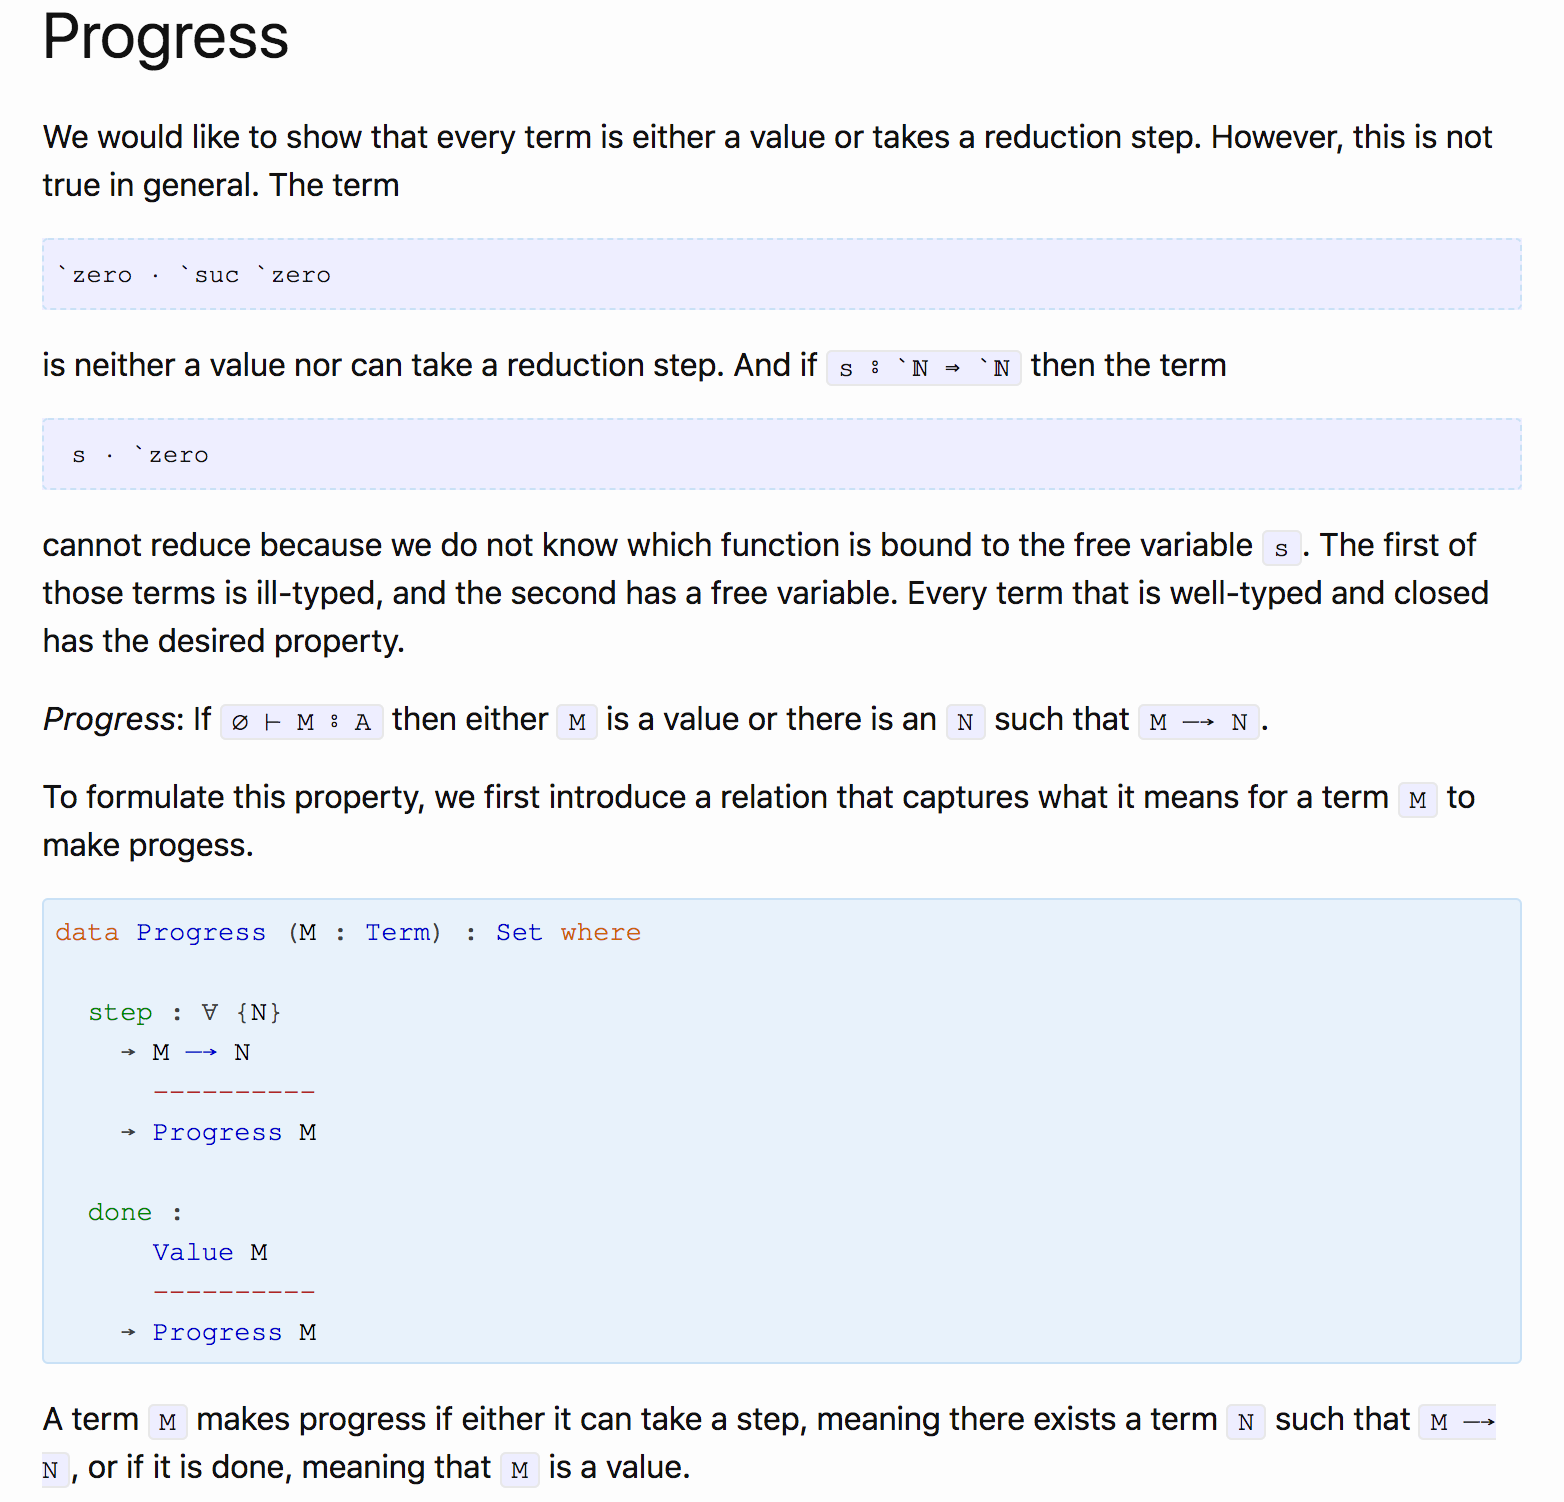
\includegraphics[width=\textwidth]{figures/plfa-progress-1.png}
  \caption{PLFA, Progress (1/2)}
  \label{fig:plfa-progress-1}
\end{figure}  

\begin{figure}[p]
  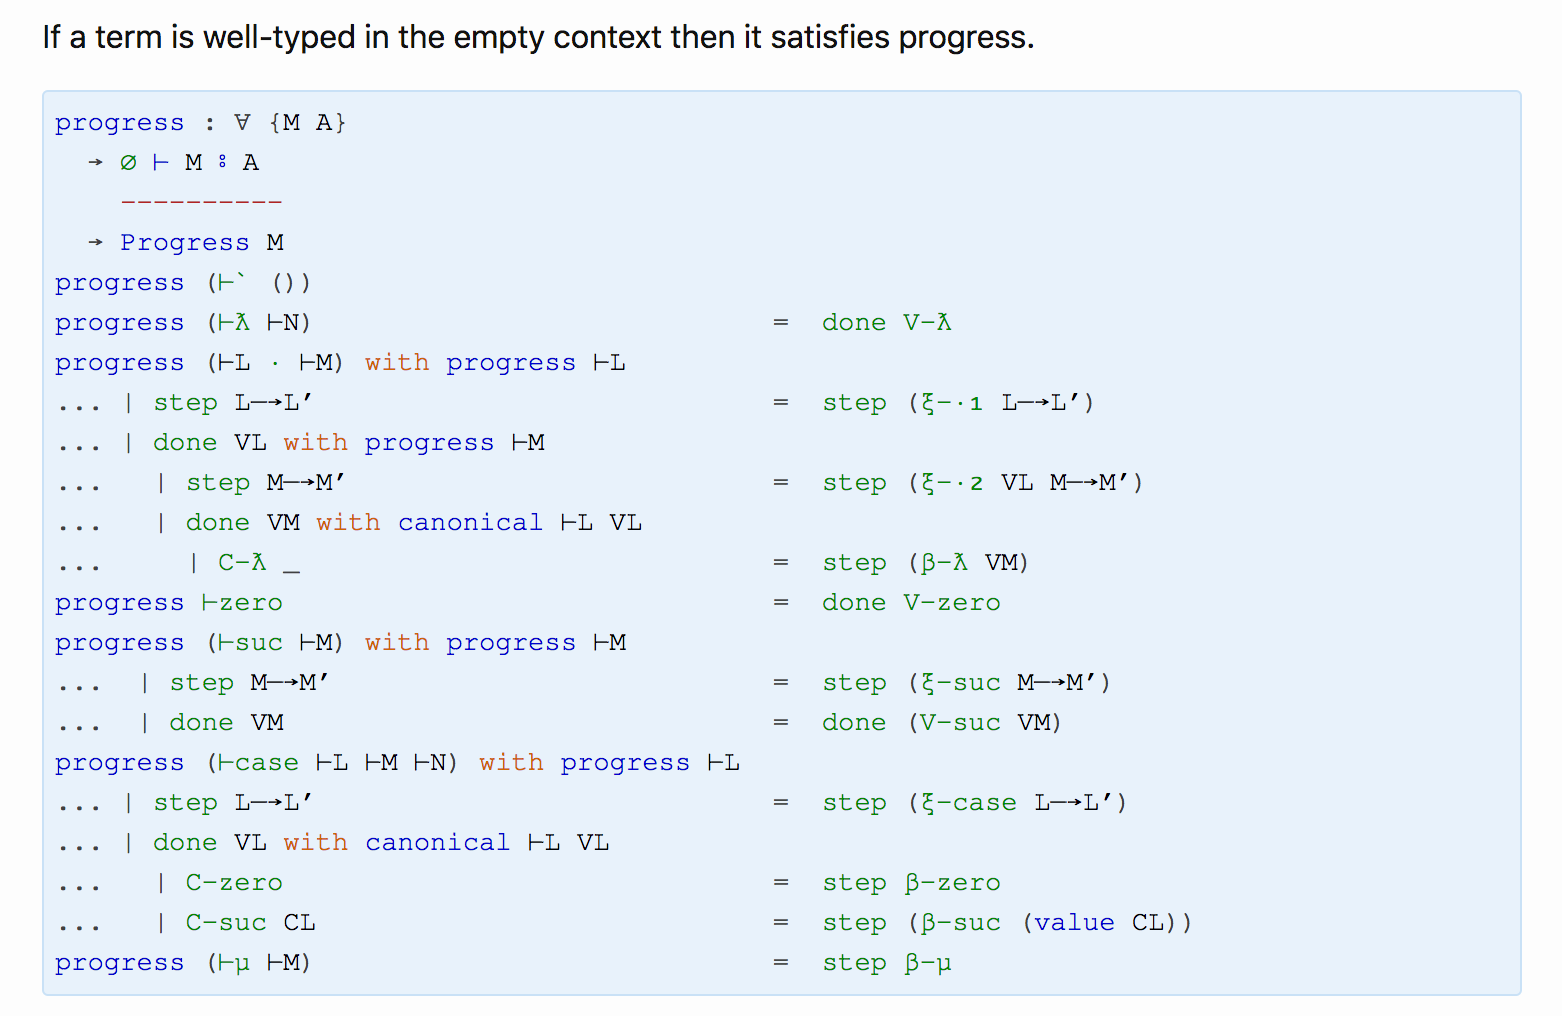
\includegraphics[width=\textwidth]{figures/plfa-progress-2.png}
  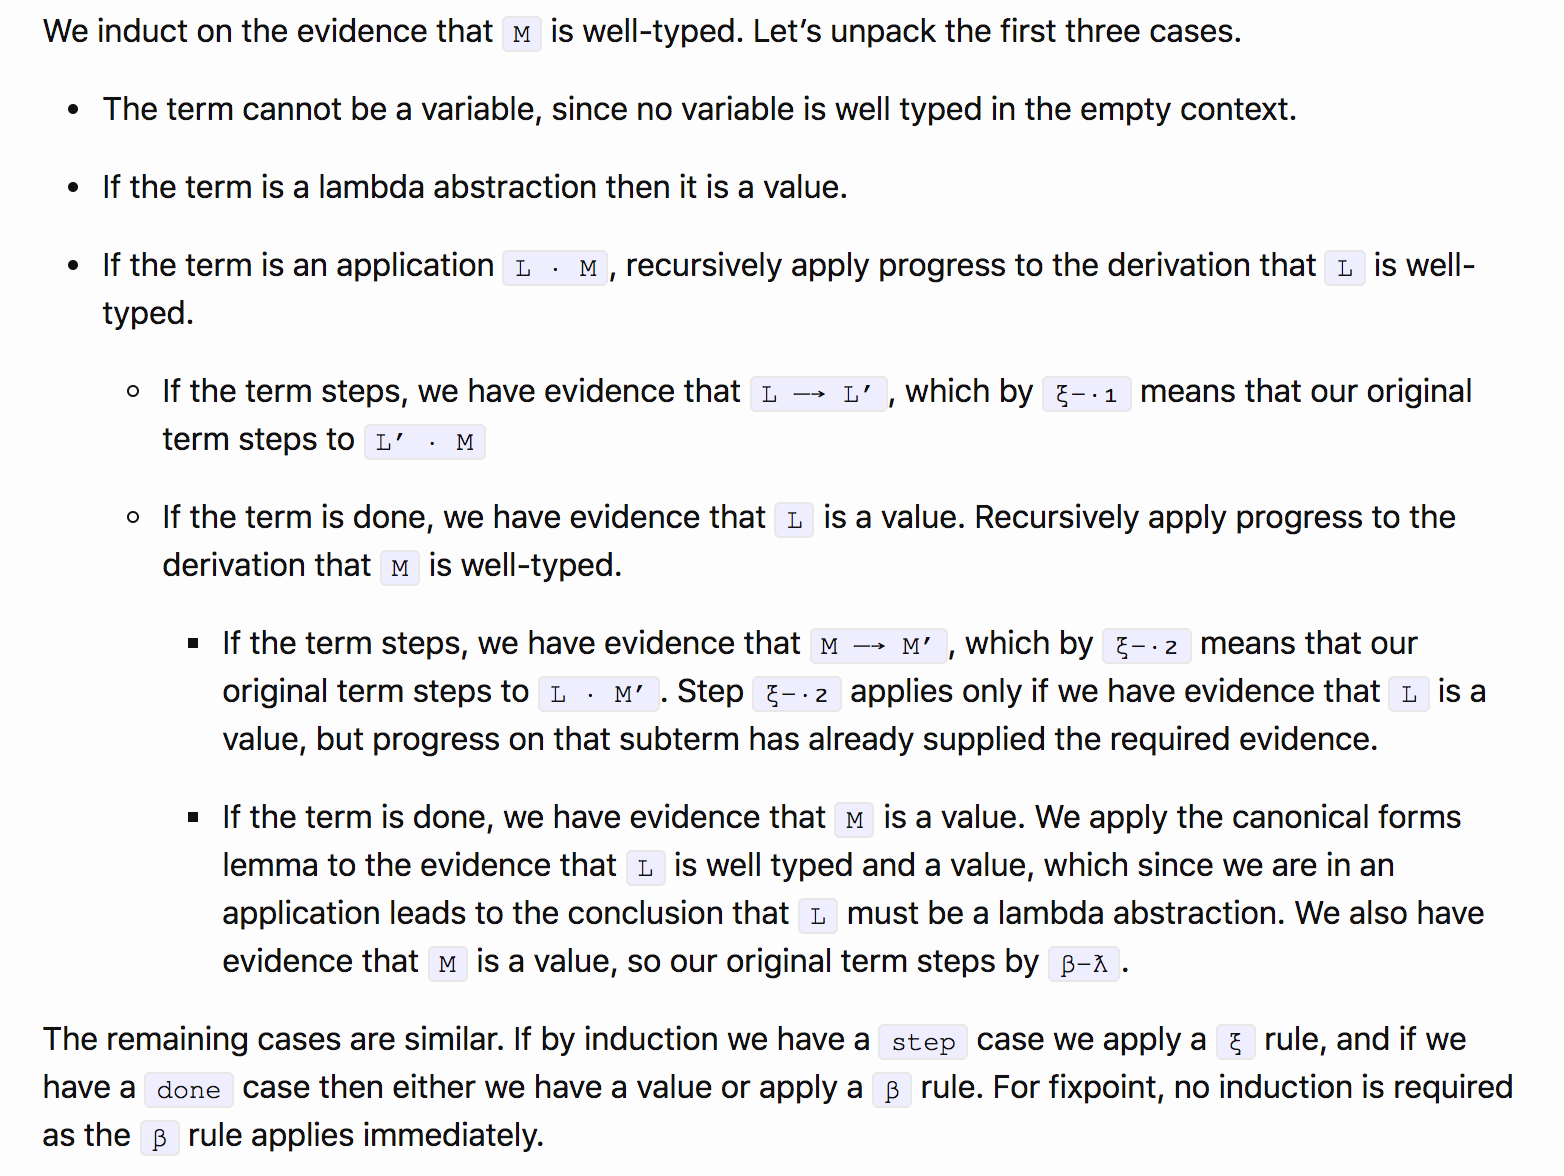
\includegraphics[width=\textwidth]{figures/plfa-progress-3a.png}
  \caption{PLFA, Progress (2/2)}
  \label{fig:plfa-progress-2}
\end{figure}  

\begin{figure}[t]
  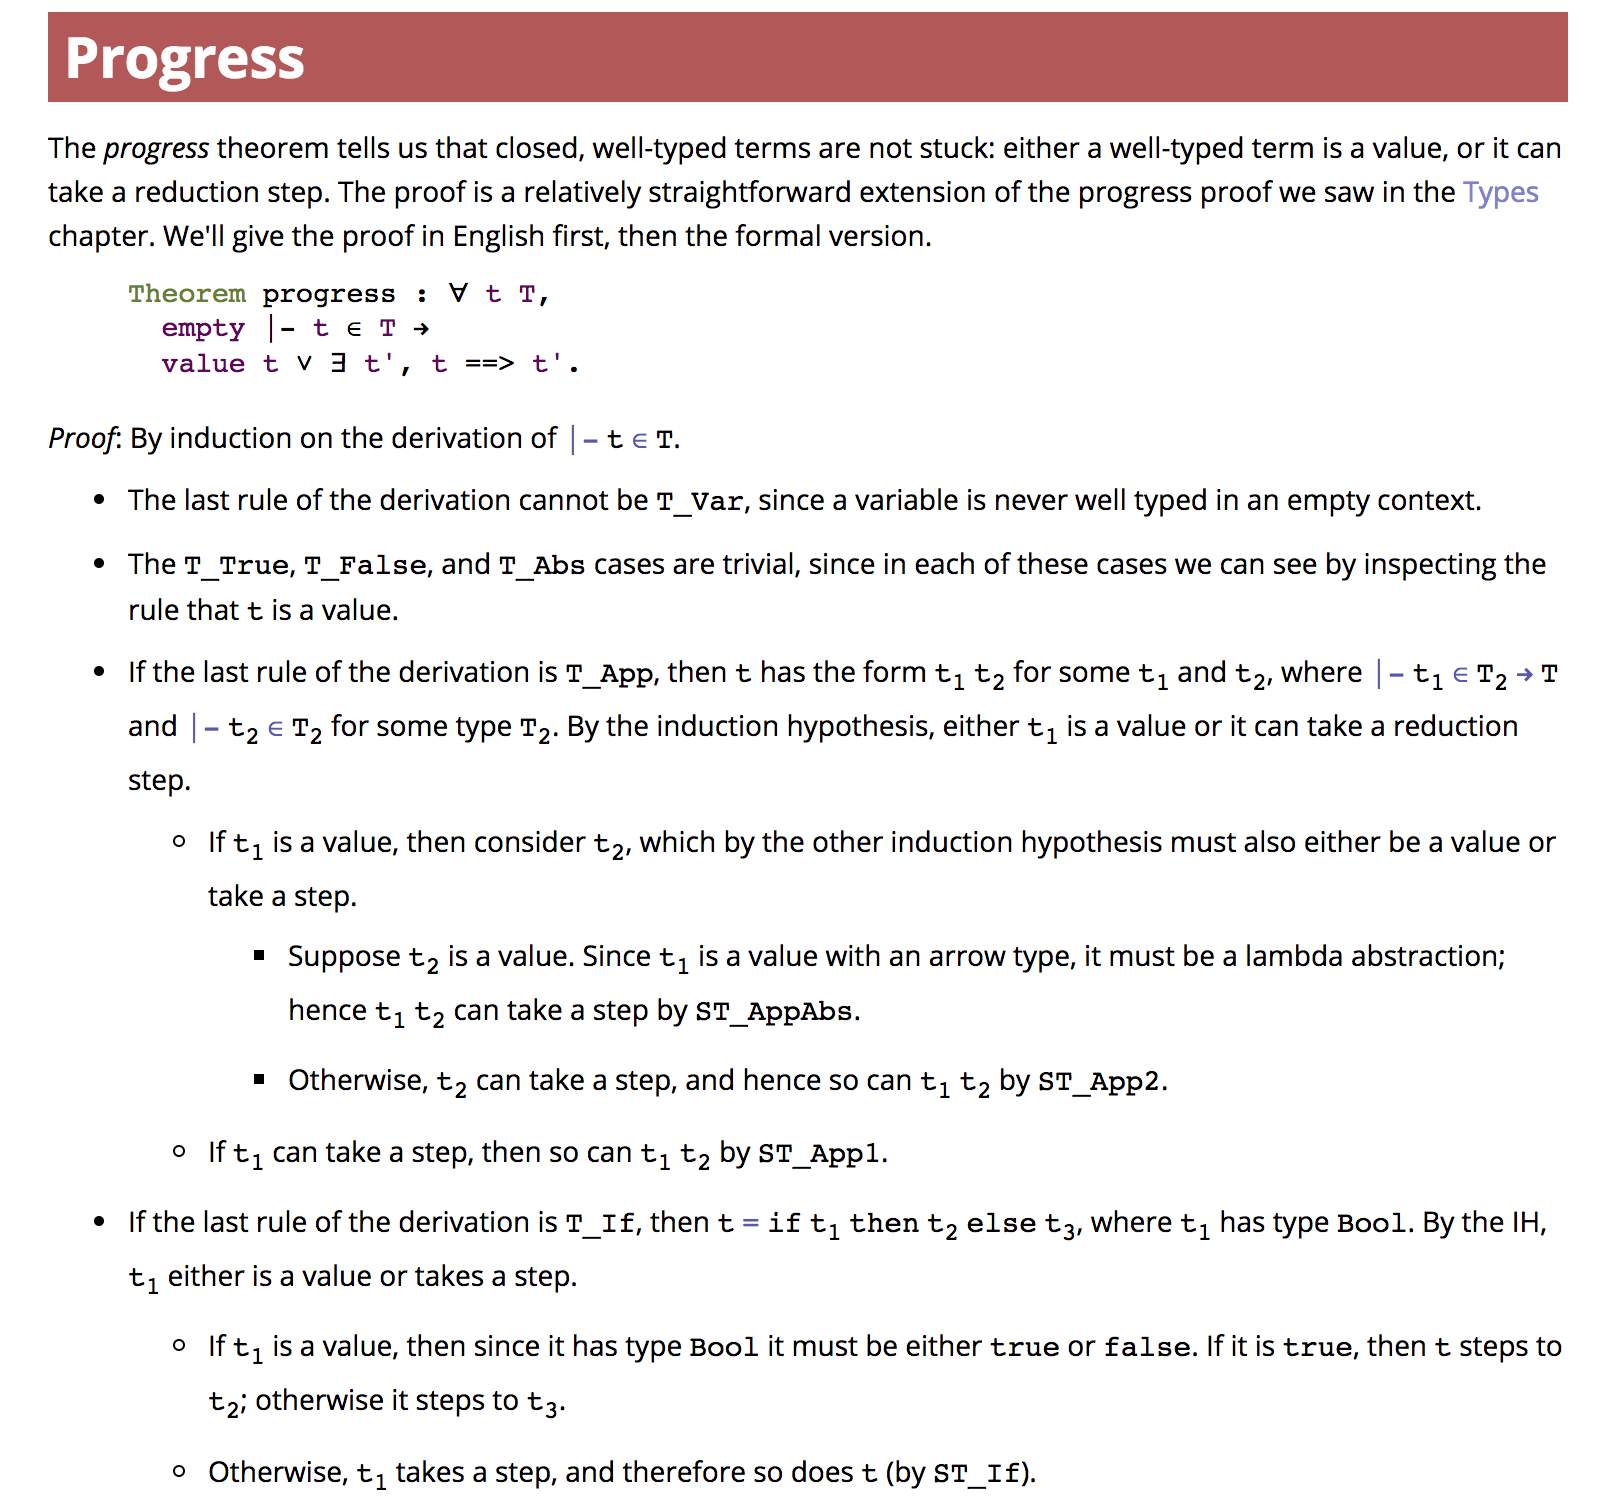
\includegraphics[width=\textwidth]{figures/sf-progress-1.png}
  \caption{SF, Progress (1/2)}
  \label{fig:sf-progress-1}
\end{figure}  

\begin{figure}[t]
  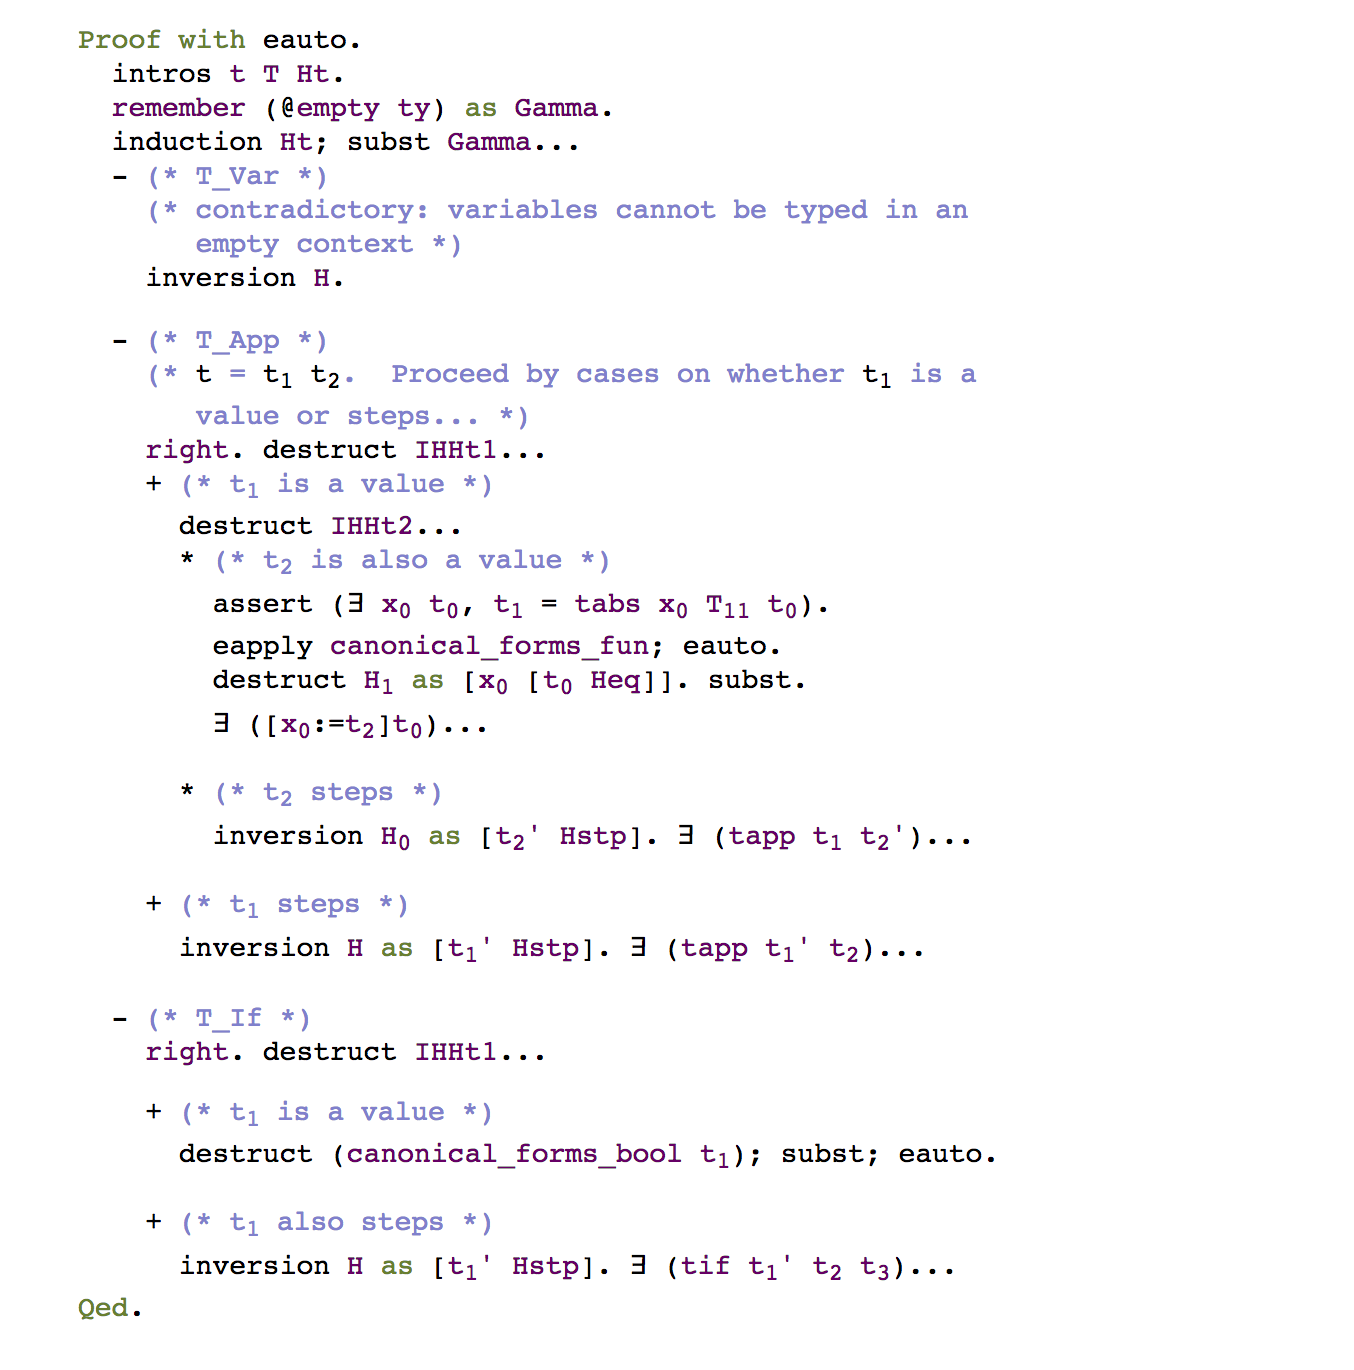
\includegraphics[width=\textwidth]{figures/sf-progress-2.png}
  \caption{SF, Progress (2/2)}
  \label{fig:sf-progress-2}
\end{figure}  

The introduction listed several reasons for preferring Agda over Coq.
But Coq tactics enable more compact proofs. Would it be possible for
PLFA to cover the same material as SF, or would the proofs
balloon to unmanageable size?

As an experiment, Philip first rewrote SF's development of simply-typed lambda
calculus (SF, Chapters Stlc and StlcProp) in Agda.  He was a newbie to Agda, and
translating the entire development, sticking as closely as possible to the
development in SF, took about two days.  We were pleased to discover that the
proofs remained about the same size.

There was also a pleasing surprise regarding the structure of the
proofs. While most proofs in both SF and PLFA are carried out by
induction over the evidence that a term is well typed, in SF the
central proof, that substitution preserves types, is carried out by
induction on terms for a technical reason
(the context is extended by a variable binding, and hence not
sufficiently ``generic'' to work well with Coq's induction tactic). In
Agda, we had no trouble formulating the same proof over evidence that
the term is well typed, and didn't even notice SF's description of the
issue until we were done.

The rest of the book was relatively easy to complete.  The closest to
an issue with proof size arose when proving that reduction is
deterministic.  There are 18 cases, one case per line.  Ten of the
cases deal with the situation where there are potentially two
different reductions; each case is trivially shown to be
impossible.  Five of the ten cases are redundant, as they just involve
switching the order of the arguments.  We had to copy the cases
suitably permuted. It would be preferable to reinvoke the proof on
switched arguments, but this would not pass Agda's termination checker
since swapping the arguments doesn't yield a recursive call on
structurally smaller arguments.  We suspect tactics could cut down the
proof significantly. We tried to compare with SF's proof that reduction
is deterministic, but failed to find that proof.

SF covers an imperative language with Hoare logic, culminating in code that
takes an imperative programme suitably decorated with preconditions and
postconditions and generates the necessary verification conditions. The
conditions are then verified by a custom tactic, where any questions of
arithmetic are resolved by the ``omega'' tactic invoking a decision procedure.
The entire exercise would be easy to repeat in Agda, save for the last step, as
Agda does not offer support for proof automation out of the box. It is 
certainly possible to implement proof automation in Agda---see, e.g., the auto
tactic by \citet{Kokke-2015}, and the collection of tactics in Ulf Norell's
\texttt{agda-prelude}\footnote{\url{https://github.com/UlfNorell/agda-prelude}}.
The standard library comes equipped with solvers for equations on monoids and
rings\footnote{\url{https://agda.github.io/agda-stdlib/Algebra.Solver.Ring.html}},
and a much improved solver for equalities on rings was recently contributed by
\citet{Kidney-2019}.
We suspect that, while Agda's automation would be up to verifying the generated
conditions, some effort would be require to implement the required custom
tactic, and a section would need to be added to the book to cover proof
automation. For the time being, we have decided to omit Hoare logic in order to
focus on lambda calculus.

To give a flavour of how the texts compare, we show the
proof of progress for simply-typed lambda calculus from both texts.
Figures~\ref{fig:plfa-progress-1} and \ref{fig:plfa-progress-2}
are taken from PLFA, Chapter Properties,
while Figures~\ref{fig:sf-progress-1} and \ref{fig:sf-progress-2}
are taken from SF, Chapter StlcProp.
Both texts are intended to be read online,
and the figures were taken by grabbing bitmaps of the text as
displayed in a browser.

PLFA puts the formal statements first, followed by informal explanation.
PLFA introduces an auxiliary relation \texttt{Progress} to capture
progress; an exercise (not shown) asks the reader to show it isomorphic
to the usual formulation with a disjunction and an existential.
Layout is used to present the auxiliary relation in inference rule form.
In Agda, any line beginning with two dashes is treated as a comment, making
it easy to use a line of dashes to separate hypotheses from conclusion
in inference rules.  The proof of proposition \texttt{progress} (the different
case making it a distinct name) is layed out carefully. The neat
indented structure emphasises the case analysis, and all right-hand
sides line-up in the same column.  Our hope as authors is that students
will read the formal proof first, and use it as a tabular guide
to the informal explanation that follows.

SF puts the informal explanation first, followed by the formal proof. The text
hides the formal proof script under an icon; the figure shows what appears when
the icon is expanded. As teachers, we were aware that students might skip the
formal proof on a first reading, and we would have to hope the students would
return to it and step through it with an interactive tool in order to make it
intelligible.  We expect the students skipped over many such proofs.  This
particular proof forms the basis for a question of the mock exam and the past
exams, so we expect most students will actually look at this one if not all the
others.

\newcommand{\ex}{\texttt{x}}
\newcommand{\why}{\texttt{y}}
\newcommand{\EL}{\texttt{L}}
\newcommand{\EM}{\texttt{M}}
\newcommand{\EN}{\texttt{N}}
\newcommand{\tee}{\texttt{t}}
\newcommand{\tick}{\texttt{\lq}}
\newcommand{\GG}{\Gamma}
\newcommand{\AY}{\texttt{A}}
\newcommand{\BE}{\texttt{B}}

(For those wanting more detail: In PLFA, variables and abstractions and
applications in the object language are written $\tick\;\ex$ and
$\lambdabar\;\ex\;{\Rightarrow}\;\EN$ and $\EL\;{\cdot}\;\EM$.  The
corresponding typing rules are referred to by ${\vdash}\tick\;()$
and ${\vdash}\lambdabar\;{\vdash}\EN$ and ${\vdash}\EL\;{\cdot}\;{\vdash}\EM$, where
${\vdash}\EL$, ${\vdash}\EM$, ${\vdash}\EN$ are the proofs that terms
$\EL$, $\EM$, $\EN$ are well typed, and `()` denotes that there cannot
be evidence that a free variable is well typed in the empty context.
It was decided to overload infix dot for readability, but not other
symbols. In Agda, as in Lisp, almost any sequence of characters is a
name, with spaces essential for separation.)

(In SF, variables and abstractions and applications in
the object language are written $\texttt{tvar}~\ex$ and
$\texttt{tabs}~\ex~\tee$ and $\texttt{tapp}~\tee_1~\tee_2$.
The corresponding typing rules are referred to as
$\texttt{T\_Var}$ and $\texttt{T\_Abs}$ and $\texttt{T\_App}$.)

Both Coq and Agda support interactive proof.  Interaction in Coq is
supported by Proof General, based on Emacs, or by CoqIDE, which
provides an interactive development environment of a sort familiar to
most students.  Interaction in Agda is supported by an Emacs mode.

In Coq, interaction consists of stepping through a proof script, at
each point examining the current goal and the variables currently in
scope, and executing a new command in the script.  Tactics are a whole
sublanguage, which must be learned in addition to the language for
expressing specifications.  There are many tactics one can invoke in
the script at each point; one menu in CoqIDE lists about one hundred
tactics one might invoke, some in alphabetic submenus.  A Coq
script presents the specification proved and the tactics executed.
Interaction is recorded in a script, which the students
may step through at their leisure.  SF contains some prose descriptions
of stepping through scripts, but mainly contains scripts that students
are encouraged to step through on their own.

In Agda, interaction consists of writing code with holes, at each
point examining the current goal and the variables in scope, and
typing code or executing an Emacs command.  The number of commands
available is much smaller than with Coq, the most important ones being
to show the type of the hole and the types of the variables in scope;
to check the code; to do a case analysis on a given variable; or to
guess how to fill in the hole with constructors or variables in scope.
An Agda proof consists of typed code.  The interaction is \emph{not}
recorded.  Students may recreate it by commenting out bits of code and
introducing a hole in their place.   PLFA contains some prose descriptions
of interactively building code, but mainly contains code that students
can read.  They may also introduce holes to interact with the code, but
we expect this will be rarer than with SF.

SF encourages students to interact with all the scripts in the text.
Trying to understand a Coq proof script without running it
interactively is a bit like understanding a chess game by reading
through the moves without benefit of a board, keeping it all in your
head.  In contrast, PLFA provides code that students can read.
Understanding the code often requires working out the types, but
(unlike executing a Coq proof script) this is often easy to do in your
head; when it is not easy, students still have the option of
interaction.

While students are keen to interact to create code, we have found they
are reluctant to interact to understand code created by others. For
this reason, we suspect this may make Agda a more suitable vehicle for
teaching.  Nate Foster suggests this hypothesis is ripe to be tested
empirically, perhaps using techniques similar to those of
\citet{Danas-et-al-2017}.

Neat layout of definitions such as that in
Figure~\ref{fig:plfa-progress-2} in Emacs requires a monospaced font
supporting all the necessary characters.  Securing one has proved
tricky. As of this writing, we use FreeMono, but it lacks a few
characters ($\typecolon$ and $\qedsymbol$) which are loaded from fonts with a different
width.  Long arrows are necessarily more than a single character wide.
Instead, we compose reduction —→ from an em dash — and an arrow →.
Similarly for reflexive and transitive closure —↠.

\section{Progress + Preservation = Evaluation}

\begin{figure}
  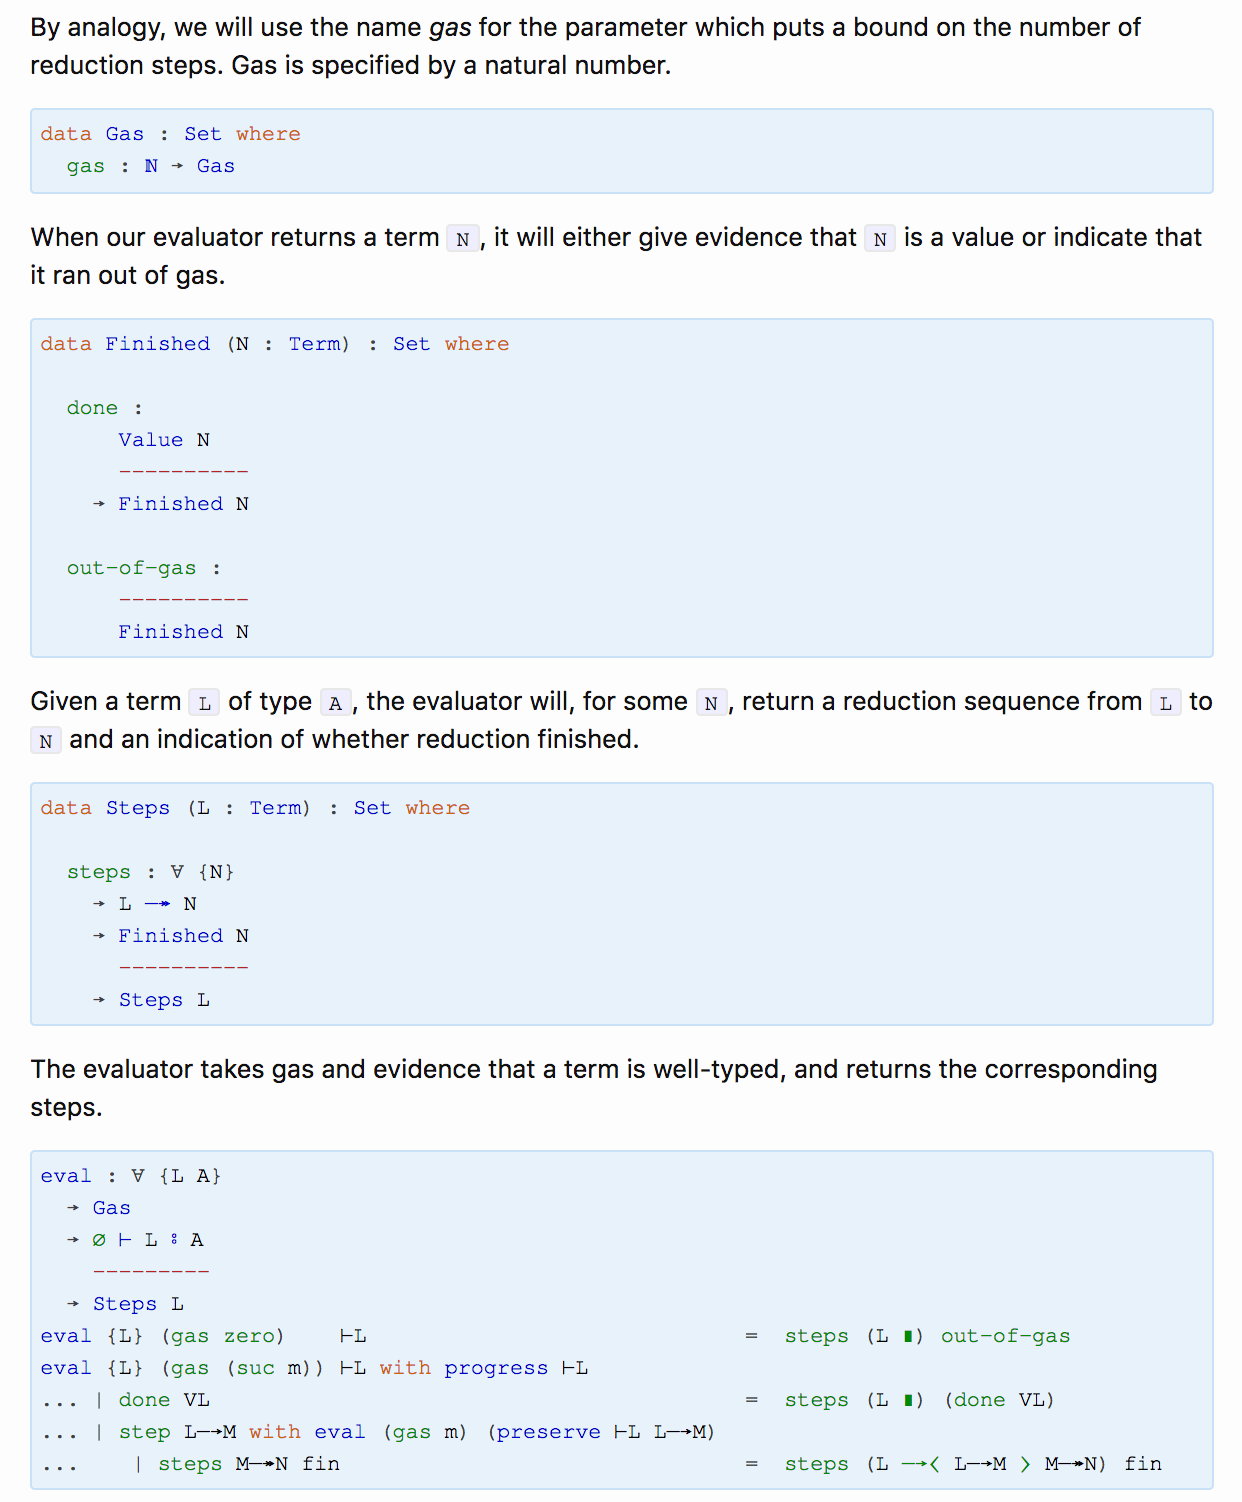
\includegraphics[width=\textwidth]{figures/plfa-eval.png}
  \caption{PLFA, Evaluation}
  \label{fig:plfa-eval}
\end{figure}  

A standard approach to type soundness used by many texts,
including SF and PLFA, is to prove progress and preservation,
as first suggested by \citet{Wright-and-Felleisen-1994}.

\begin{theorem}[Progress] Given term $M$ and type $A$ such that
$\emptyset \vdash M : A$ then either $M$ is a value or
$M \longrightarrow N$ for some term $N$.
\end{theorem}

\begin{theorem}[Preservation] Given terms $M$ and $N$ and type $A$
such that $\emptyset \vdash M : A$ and $M \longrightarrow N$, then
$\emptyset \vdash N : A$.  \end{theorem}

A consequence is that when a term reduces to a value it retains
the same type.  Further, well-typed terms don't get stuck:
that is, unable to reduce further but not yet reduced to a value.
The formulation neatly accommodates the case of non-terminating
reductions that never reach a value.

One useful by-product of the formal specification of a programming
language may be a prototype implementation of that language.  For
instance, given a language specified by a reduction relation, such
as lambda calculus, the prototype might accept a term and apply reductions
to reduce it to a value.  Typically, one might go to some extra work to
create such a prototype.  For instance, SF introduces a \texttt{normalize}
tactic for this purpose.  Some formal methods frameworks, such as
Redex \citep{Felleisen-et-al-2009} and K \citep{Rosu-Serbanuta-2010},
advertise as one of their advantages that they can generate
a prototype from descriptions of the reduction rules.

% new
Philip had been exposed to the work of the K team, as both consulted
for IOHK, a cryptocurrency firm.  This put us keenly in mind of the
need for animation; Philip sometime referred to this as ``K-envy'' or
``Redex-envy''.

% TODO: rewrite use of 'Philip' to reflect all authors?
Philip was therefore surprised to realise that any constructive proof of
progress and preservation \emph{automatically} gives rise to such a
prototype.  The input is a term together with evidence the term is
well-typed.  (In the inherently-typed case, these are the same thing.)
Progress determines whether we are done, or should take another step;
preservation provides evidence that the new term is well-typed, so we
may iterate. In a language with guaranteed termination, we cannot
iterate forever, but there are a number of well-known techniques to
address that issue; see, e.g., \citet{Bove-and-Capretta-2001},
\citet{Capretta-2005}, or \citet{McBride-2015}.
We use the simplest, similar to McBride's \emph{petrol-driven} (or
\emph{step-indexed}) semantics: provide a maximum number of steps to
execute; if that number proves insufficient, the evaluator returns the
term it reached, and one can resume execution by providing a new
number.

Such an evaluator from PLFA is shown in Figure~\ref{fig:plfa-eval},
where (inspired by cryptocurrencies) the number of steps
to execute is referred to as \emph{gas}. All of the example reduction
sequences in PLFA were computed by the evaluator and then edited to
improve readability; in addition, the text includes examples of
running the evaluator with its unedited output.

It is immediately obvious that progress and preservation make it
trivial to construct a prototype evaluator, and yet we cannot find such
an observation in the literature nor mentioned in an introductory
text.  It does not appear in SF, which introduces a specialised
\texttt{normalise} tactic instead.  A plea
to the Agda mailing list failed to turn up any prior mentions.
The closest related observation we have seen in the published
literature is that evaluators can be extracted from proofs of
normalisation \citep{Berger-1993,Dagand-and-Scherer-2015}.

% NEW
Some researchers are clearly familiar with the connection between
progress and preservation and animation.  In private correspondence,
Bob Harper referred to it as the \emph{pas de deux}, a dance between
progress, which takes well-typing to a step, and preservation, which
takes a step back to well-typing.  Nonetheless, neither the technique
nor the appealing terminology, appears in \citet{Harper-2016}.  The
appeal to the Agda mailing list bore late fruit: Oleg Kiselyov
directed me to unpublished remarks on his web page where he uses the
name \texttt{eval} for a proof of progress and notes ``the very proof
of type soundness can be used to evaluate sample expressions''
\citep{Kiselyov-2009}.  Nonetheless, as of this writing, we still have
not located a mention in the published literature.

% NEW
There are places in the literature where one might expect a remark on
the relation between progress and preservation and animation---but no
such remark appears.  In the PoplMark Challenge
\citep{Ayedemir-et-al-2005}, Challenge~2A is to prove progress and
preservation for System F$_{<:}$, while Challenge~3 is to prove
animation for the same system. Nowhere do the authors indicate that in
an intuitionistic logic these are essentially the same problem.
\cite{Owens-et-al-2016}, when discussing extraction of animators for
small-step semantics, mention Redex and K, but no other possibilities.
We hope the stress in PLFA on the fact that in an intuitionistic
setting progress and preservation imply animation will mean that the
connection becomes more widely known.






\section{Inherent typing is golden}

\begin{figure}[p]
  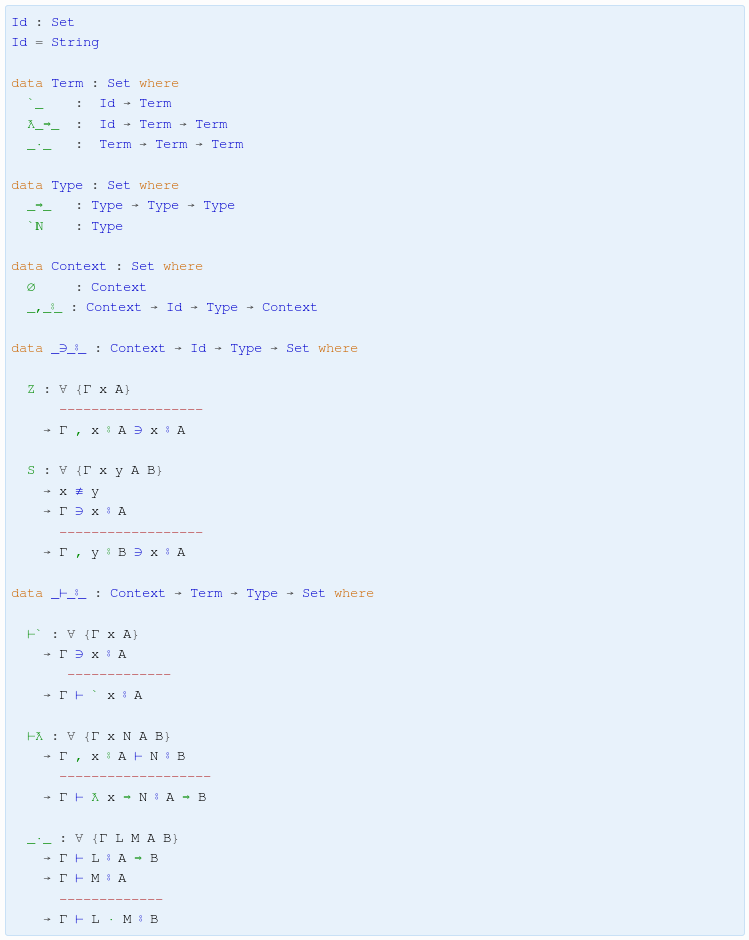
\includegraphics[width=\textwidth]{figures/raw.png}
  \caption{Raw approach in PLFA}
  \label{fig:raw}
\end{figure}  

\begin{figure}[t]
  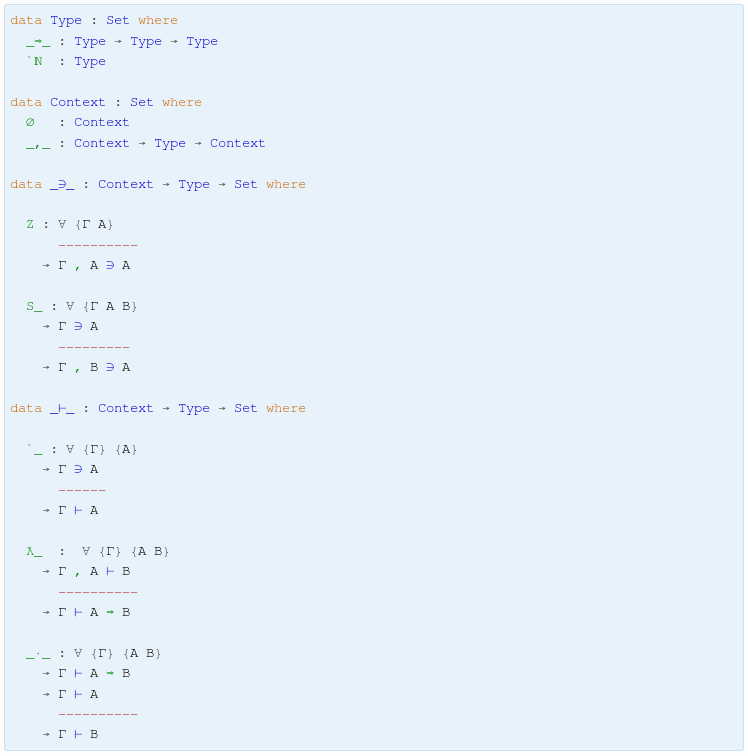
\includegraphics[width=\textwidth]{figures/inherent.png}
  \caption{Inherent approach in PLFA}
  \label{fig:inherent}
\end{figure}  

% TODO: consider rewriting this?
The second part of PLFA first discusses two different approaches to
modeling simply-typed lambda calculus.  It first presents raw
terms with named variables and a separate typing relation and
then shifts to inherently-typed terms with de Bruijn indices.
Before writing the text, Philip had thought the two approaches
complementary, with no clear winner.  Now he is convinced that the
inherently-typed approach is superior.

Figure~\ref{fig:raw} presents the raw approach.
It first defines $\texttt{Id}$, $\texttt{Term}$,
$\texttt{Type}$, and $\texttt{Context}$, the abstract syntax
of identifiers, raw terms, types, and contexts.
It then defines two judgments,
$\GG\:{\ni}\:\ex\:{\typecolon}\:\AY$ and
$\GG\:{\vdash}\:\EM\:{\typecolon}\:\AY$,
which hold when under context $\GG$ the variable $\ex$
and the term $\EM$ have type $\AY$, respectively.

Figure~\ref{fig:inherent} presents the inherent approach.
It first defines $\texttt{Type}$ and $\texttt{Context}$, the abstract syntax
of types and contexts, of which the first is as before and the second is
as before with identifiers dropped.  In place of the two judgments,
the types of variables and terms are indexed by a context and a type,
so that $\GG\:{\ni}\:\AY$ and $\GG\:{\vdash}\:\AY$ denote
variables and terms, respectively, that under context $\GG$ have type $\AY$.
The indexed types closely resemble the previous judgments:
we now represent a variable or a term by the proof that it is well typed.
In particular, the proof that a variable is well typed in the raw approach
corresponds to a de Bruijn index in the inherent approach.

The raw approach requires more lines of code than the inherent approach.  The
separate definition of raw terms is not needed in the inherent approach; and one
judgment in the raw approach needs to check that $\ex \not\equiv \why$, while
the corresponding judgment in the inherent approach does not.  The difference
becomes more pronounced when including the code for substitution, reductions,
and proofs of progress and preservation.  In particular, where the raw approach
requires one first define substitution and reduction and then prove they
preserve types, the inherent approach establishes substitution at the same time
it defines substitution and reduction.

Stripping out examples and any proofs that appear in one but not the other (but
could have appeared in both), the full development in PLFA for the raw approach
takes 451 lines (216 lines of definitions and 235 lines for the proofs) and the
development for the inherent approach takes 275 lines (with definitions and
proofs interleaved).  We have 451 / 235 = 1.64, close to the golden ratio.

The inherent approach also has more expressive power.  The raw
approach is restricted to substitution of one variable by a closed
term, while the inherent approach supports simultaneous substitution
of all variables by open terms, using a pleasing formulation due to
\citet{McBride-2005}, inspired by \citet{Goguen-and-McKinna-1997} and
\citet{Altenkirch-and-Reus-1999} and described in
\citet{Allais-et-al-2017}. In fact, we did manage to write a variant of
the raw approach with simultaneous open substitution along the lines
of McBride, but the result was too complex for use in an introductory
text, requiring 695 lines of code---more than the total for the other
two approaches combined.
% TODO: is this still available somewhere in extra/?

The text develops both approaches because the raw approach is more
familiar, and because placing the inherent approach first would
lead to a steep learning curve.  By presenting the more long-winded
but less powerful approach first, students can see for themselves the
advantages of de Bruijn indices and inherent types.

There are actually four possible designs, as the choice of named
variables vs de Bruijn indices, and the choice of raw vs
inherently-typed terms may be made independently.  There are synergies
between the two.  Manipulation of de Bruijn indices can be notoriously
error-prone without inherent-typing to give assurance of correctness.
In inherent typing with named variables, simultaneous substitution by
open terms remains difficult.

The benefits of the inherent approach 
are well known to some. The technique was introduced by
\citet{Altenkirch-and-Reus-1999}, and widely used elsewhere,
notably by \citet{Chapman-2009} and \citet{Allais-et-al-2017}.
Philip is grateful to David Darais for bringing it to his attention.


\section{Teaching experience}

Philip now has five years of experience teaching from SF and one year
teaching from PLFA.  To date, he has taught three courses from PLFA.
\begin{itemize}
\item
  University of Edinburgh, September--December 2018 (with teaching
  assistance from Wen and Chad Nester); twenty two-hour slots,
  comprising one hour of lecture followed by one hour of lab. Ten
  students completed the course, fourth-year undergraduates and
  masters.  The course covered Parts~I and~II of PLFA.

\item
  Pontifícia Universidade Católica do Rio de Janeiro (PUC-Rio),
  March--July 2019, hosted by Roberto Ieuramalischy; ten three-hour
  slots, comprising two hours of lecture followed by one hour of lab.
  Ten students completed the course, mostly doctoral students.  The
  course covered Parts~I and~II of PLFA, save students read chapter
  Lists on their own, and chapter Bisimilarity was skipped.

\item
  University of Padova, June 2018, hosted by Maria Emilia Maietti; two
  three-hour slots, comprising two hours of lecture followed by one
  hour of lab.  Thirty undergraduate students sat the course, which
  covered chapters Naturals, Induction, and Relations.
    
\end{itemize}
In addition, David Darais at University of Vermont and John Leo at
Google Seattle have taught from PLFA.

Exercises in PLFA are classified in three ways.
\begin{itemize}
\item
  Exercises labelled “(recommended)” are the ones students are
  required to do in the classes taught at Edinburgh and PUC-Rio.

\item
  Exercises labelled “(stretch)” are there to provide an extra
  challenge. Few students do all of these, but most attempt at least a
  few. 

\item   
  Exercises without a label are included for those who want extra
  practice.  To Philip's surprise, students at PUC-Rio completed
  quite a few of these.
\end{itemize}
Students are expected to complete coursework for all of the
required questions in the text, optionally doing any stretch or
unlabelled exercises. Coursework also includes a ``mock mock''
exam, as described below.

The mark for the course is based on coursework and a final-exam,
weighted 1/4 for coursework and 3/4 for the final exam.  The weighting
for coursework is designed to be high enough to encourage students to
do it (they all do), but not so high as to encourage cheating.
Students are encouraged to help each other with coursework.

The final-exam is two hours online. Students have access to the Agda
proof assistant to check their work.  At Edinburgh, students use
computers with a special exam operating system that disables access
to the internet.  Students are given access to the text of PLFA,
the Agda standard libraries, and the Agda language reference manual,
but no other materials.

Students must answer question 1 on the exam, and one of questions 2 or
3.  Question 1 gives predicates over a data structure, such lists or
trees, to be formalised in Agda, and a theorem relating the
predicates, to be formalised and proved in Agda.  Question 2 gives the
students the intrinsic formulation of lambda calculus from chapter
DeBruijn, which they must extend with a described language feature.
Question 3 give the students the the bidirectional type inferencer
from chapter Inference, which they must extend with a described
language feature.

Because the course is taught using a proof assistant, it is important
that students have access to a proof assistant during the exam.
Students are told in advance that they are expected to get perfect on
the exam, and that they will have to study hard to achieve this level.
Given that the goal of formal methods is to avoid error, we believe a
pedagogical purpose is served by telling the students that they are
expected to achieve perfection and making it possible for them to do
so.  Students are given two opportunities to practice in the run up to
the exam, a `mock' exam given in class under exam conditions (two
hours online), and before that a `mock mock' exam as coursework (in
their own time, encouraged to ask questions, tasked to do all three
questions rather than two of three).

For the courses run at Edinburgh and PUC-Rio, the scores vary
widely on the mock, but all students achieve perfection on the
exam.  (The one exception was a PUC-Rio student who did not attend
classes or sit the mock.)  Similar results were achieved at Edinburgh
over the previous five years, using SF as the course textbook and Coq
as the proof assistant.  We consider these results a tribute to the
students' ability to study and learn.


\section{Software}

The book is written using a combination of literate Agda and Markdown.  At the
time of writing, the book is published using GitHub Pages and the Jekyll static
site generator.  The book is open source---the source is currently also hosted
on GitHub, under a Creative Commons CC-BY license.  The open-source aspect is
important---as the book is written in literate Agda, it is essential that anyone
can download and execute the source.

We maintain a number of tools, which play various roles in rendering the book in
all its ``glorious clickable HTML''. We render the literate Agda to highlighted
HTML using Agda's HTML backend. In addition to highlighting, this inserts
clickable links, linking each constructor and function to the site of its
definition.  However, the links Agda inserts are local and don't match the
structure of the book.  We maintain a script, \texttt{highlight.sh}, which fixes
these links, rerouting links to the standard library to the online version, and
correcting links to local modules.

(Before the release of Agda 2.6, Agda did not support highlighting embedded
literate code using HTML.  To address this, we wrote \texttt{agda2html}, a tool
which rewrote the output of Agda's HTML highlighter to accomplish this. This
tool had much more functionality, including the fixing of links as outlined
above, the stripping of implicit arguments to achieve a Haskell-like look, and
the support for new Markdown constructs for linking to Agda names. However,
Agda 2.6 has incorporated almost all of this functionality.)

The book is built, tested, and published after each commit, using Travis CI, a
web service for continuous integration.  The means that the book is constantly
changing.  To accommodate those who want a more stable version, e.g., for
teaching, we maintain a stable version of the book at
\begin{center}
  \url{http://plfa.inf.ed.ac.uk/stable}
\end{center}
The stable version of the book is only updated much less frequently, and updates
are announced.

We maintain a tool called, simply, \texttt{acknowledgements}, which uses
the GitHub API to automatically extract a list of contributors to the book, and
add them to the Acknowledgements page, each time the book is published.  We
consider anyone who has sent a successful pull requests a contributor, and sort
contributors in the acknowledgments by the number of accepted requests.
Arguably, a different metric, such as total number of affected lines, might be
more appropriate, though any solution may have its flaws.

\section{Conclusion}

One sign of a successful publication is that it will attract a few letters from
readers who have noticed typos or other problems.  An unexpected benefit of
publishing on GitHub is that to date forty-one readers have sent a total of
\emph{two hundred seventy-five} pull requests.  Most of these fix typos, but a
fair number make more substantial improvements.

There is much left to do!  We hope others may be inspired to join us and expand
the book.

\paragraph{Acknowledgments}

For inventing ideas on which PLFA is based, and for hand-holding, many thanks to
Conor McBride, James McKinna, Ulf Norell, and Andreas Abel.  For showing how
much more compact it is to avoid raw terms, thanks to David Darais.  For
inspiring our work by writing SF, thanks to Benjamin Pierce and his coauthors.
For comments on a draft of this paper, an extra thank you to James McKinna, Ulf
Norell, Andreas Abel, and Benjamin Pierce. This research was supported by EPSRC
Programme Grant EP/K034413/1.


\section*{References}

\bibliographystyle{elsarticle-harv}
\bibliography{PLFA}

\end{document}



% LocalWords:  Agda adr Kokke Siek Wadler Woodlawn Bloomington Coq et
% LocalWords:  PLFA evaluator normalise programme programmes al Huet
% LocalWords:  ICFP subst Bove Mixfix de Janeiro summarising favour
% LocalWords:  organised formalising Colour Gonthier CompCert Kastner
% LocalWords:  SEL honours formalisms monus associativity reflexivity
% LocalWords:  commutativity equational of's Isomorphism isomorphism
% LocalWords:  extensionality disjunction intuitionistic existentials
% LocalWords:  Booleans booleans monoid specialisation PCF Plotkin EP
% LocalWords:  fixpoint DeBruijn Bruijn indices Bisimulation Untyped
% LocalWords:  bisimulation normalisation untyped Abadi Barendregt
% LocalWords:  Rosser Tait Schafer Tebbi Smolka Pfenning Denotational
% LocalWords:  denotational Engeler lookup Compositional congruences
% LocalWords:  compositional compositionality denotationally Hoare
% LocalWords:  refactoring subtyping Appel QuickChick formalise SF's
% LocalWords:  Stlc StlcProp Coq's reinvoke Agda's postconditions Ulf
% LocalWords:  flavour layed emphasises tvar tapp CoqIDE sublanguage
% LocalWords:  submenus Danas monospaced FreeMono Felleisen Redex
% LocalWords:  Rosu Serbanuta realise Capretta cryptocurrencies Oleg
% LocalWords:  evaluators Dagand Scherer Kiselyov eval Goguen McKinna
% LocalWords:  Altenkirch Reus Allais Darais Conor Norell Andreas
% LocalWords:  EPSRC
